%
% Niniejszy plik stanowi przykład formatowania pracy magisterskiej na
% Wydziale MIM UW.  Szkielet użytych poleceń można wykorzystywać do
% woli, np. formatujac wlasna prace.
%
% Zawartosc merytoryczna stanowi oryginalnosiagniecie
% naukowosciowe Marcina Wolinskiego.  Wszelkie prawa zastrzeżone.
%
% Copyright (c) 2001 by Marcin Woliński <M.Wolinski@gust.org.pl>
% Poprawki spowodowane zmianami przepisów - Marcin Szczuka, 1.10.2004
% Poprawki spowodowane zmianami przepisow i ujednolicenie
% - Seweryn Karłowicz, 05.05.2006
% Dodanie wielu autorów i tłumaczenia na angielski - Kuba Pochrybniak, 29.11.2016

% dodaj opcję [licencjacka] dla pracy licencjackiej
% dodaj opcję [en] dla wersji angielskiej (mogą być obie: [licencjacka,en])
\documentclass[licencjacka,en]{pracamgr}
\usepackage{hyperref}
\usepackage{mathtools}
\usepackage{amssymb}
\newcommand{\bibDownloadDate}{\today}
\usepackage{tikz}
\usepackage{pgfplots}
% \usepackage{float}
%\usepackage{caption}
\usepackage[font=small,labelfont=bf]{caption}

\pgfplotstableread[row sep=\\,col sep=&]{
		epochs & training & validation \\ 
		1 & 1.02 & 0.41 \\
		2 & 0.45 & 0.29 \\
		3 & 0.33 & 0.26 \\
		4 & 0.26 & 0.24 \\
		5 & 0.22 & 0.22 \\
		6 & 0.18 & 0.21 \\
		7 & 0.16 & 0.21 \\
		8 & 0.14 & 0.20 \\
		9 & 0.13 & 0.21 \\
		10 & 0.11 & 0.21 \\
		11 & 0.10 & 0.22 \\
		12 & 0.10 & 0.22 \\
		13 & 0.09 & 0.22 \\
	}\amp
	
	\pgfplotstableread[row sep=\\,col sep=&]{
		epochs & training & validation \\ 
		1 & 0.86 & 0.33 \\
		2 & 0.39 & 0.26 \\
		3 & 0.30 & 0.23 \\
		4 & 0.25 & 0.21 \\
		5 & 0.21 & 0.20 \\
		6 & 0.19 & 0.19 \\
		7 & 0.17 & 0.19 \\
		8 & 0.15 & 0.18 \\
		9 & 0.14 & 0.18 \\
		10 & 0.13 & 0.18 \\
		11 & 0.12 & 0.176 \\
		12 & 0.11 & 0.18 \\
		13 & 0.11 & 0.18 \\
	}\norm
	
\pgfplotstableread[row sep=\\,col sep=&]{
	epochs & training \\
	1   &  4.79 \\
	30   &  2.91 \\
	60   &  2.90 \\
	90   &  2.87 \\
	120  &  2.87 \\
	150  &  2.87 \\
	180  &  2.87 \\
	210  &  2.86 \\
	240  &  2.35 \\
	270 &  1.95 \\
	300 &  1.84 \\
	330 &  1.77 \\
	360 &  1.72 \\
	390 &  1.69 \\
	420 &  1.66 \\
	450 &  1.65 \\
	480 &  1.62 \\
	510 &  1.61 \\
	540 &  1.59 \\
	570 &  1.64 \\
	600 &  1.60 \\
}\first

\newcommand{\todoplot}[1]{
	\ \\
	\noindent%
	\begin{minipage}{\linewidth}% to keep image and caption on one page
		\makebox[\linewidth]{%        to center the image
			\begin{tikzpicture}
			\begin{axis}[
			ymin = 0, ymax = 5,
			xmin = 0, xmax = 600,
			minor y tick num = 4,
			minor x tick num = 1,
			ymajorgrids = true,
			grid style = dashed,
			scaled x ticks = false,
			xlabel = TODO,
			ylabel = TODO,
			legend pos=outer north east,
			no markers
			]
			\addplot table[x=epochs,y=training]{\first};
			\addlegendentry{TODO}
			
			\end{axis}
			\end{tikzpicture}
		}\captionof{figure}{#1}\label{diag:time}     
	\end{minipage}
}

% Dane magistrantów:
\autor{Piotr Ambroszczyk}{385090}
\autori{Łukasz Kondraciuk}{385775}
\autorii{Wojciech Przybyszewski}{386044}
\autoriii{Jan Tabaszewski}{386319}

\title{Deep Learning for Speech Recognition -- Deep Speech 2}
\titlepl{Rozpoznawanie mowy metodami głębokiego uczenia -- Deep Speech 2}

%\tytulang{An implementation of a difference blabalizer based on the theory of $\sigma$ -- $\rho$ phetors}

%kierunek:
% - matematyka, informacyka, ...
% - Mathematics, Computer Science, ...
\kierunek{Computer Science}

% informatyka - nie okreslamy zakresu (opcja zakomentowana)
% matematyka - zakres moze pozostac nieokreslony,
% a jesli ma byc okreslony dla pracy mgr,
% to przyjmuje jedna z wartosci:
% {metod matematycznych w finansach}
% {metod matematycznych w ubezpieczeniach}
% {matematyki stosowanej}
% {nauczania matematyki}
% Dla pracy licencjackiej mamy natomiast
% mozliwosc wpisania takiej wartosci zakresu:
% {Jednoczesnych Studiow Ekonomiczno--Matematycznych}

% \zakres{Tu wpisac, jesli trzeba, jedna z opcji podanych wyzej}

% Praca wykonana pod kierunkiem:
% (podać tytuł/stopień imię i nazwisko opiekuna
% Instytut
% ew. Wydział ew. Uczelnia (jeżeli nie MIM UW))
\opiekun{dr Janina Mincer-Daszkiewicz \\
	Instytut Informatyki\\
}

% miesiąc i~rok:
\date{June 2019}

%Podać dziedzinę wg klasyfikacji Socrates-Erasmus:
\dziedzina{
	%11.0 Matematyka, Informatyka:\\
	%11.1 Matematyka\\
	%11.2 Statystyka\\
	11.3 Informatyka\\
	%11.4 Sztuczna inteligencja\\
	%11.5 Nauki aktuarialne\\
	%11.9 Inne nauki matematyczne i informatyczne
}

%Klasyfikacja tematyczna wedlug AMS (matematyka) lub ACM (informatyka)
\klasyfikacja{D. Software\\
	%D.127. Blabalgorithms\\
	%D.127.6. Numerical blabalysis
}

% Słowa kluczowe:
\keywords{Deep Speech, ASR, neural networks, machine learning, Python, PyTorch, NVIDIA, RNN, multi-GPU, mixed precision training}

% Tu jest dobre miejsce na Twoje własne makra i~środowiska:
\newtheorem{defi}{Definicja}[section]

% koniec definicji

\begin{document}
	\maketitle
	
	%tu idzie streszczenie na strone poczatkowa
	\begin{abstract}
		The authors of this thesis focus on implementing scripts for training Deep Speech 2 model for Automatic Speech Recognition. We try to reproduce results obtained by Baidu Research in End-to-End Speech Recognition paper \cite{DS2} using PyTorch framework and techniques for speeding up computations on GPUs -- training in mixed precision and multi-GPU scaling. We provide fully trained models for English language together with statistics about how changing hyperparameters and architecture impacts performance and accuracy of the model.
	\end{abstract}
	
	\tableofcontents
	%\listoffigures
	%\listoftables
	
	\chapter*{Introduction}
	\addcontentsline{toc}{chapter}{Introduction}
	Transcription of spoken language is a crucial problem for many areas of a modern technology industry. Being able to communicate with electronic devices not only by touching them, but also by talking to them is an important goal for IT companies. Such devices are more user-friendly and undoubtedly beneficial for everybody. Various solutions were proposed for speech recognition, and many of them use complex algorithms (e.g. Hidden Markov Models) \cite{DS1}. However, it has been shown that the best accuracy can be achieved with Automatic Speech Recognition (ASR) models based on neural networks \cite{DS2}.
	
	Our thesis concentrates on implementing state of the art ASR model Deep Speech 2 (DS2) described in \cite{DS2}, and we realize it with the support of NVIDIA Corporation. Authors of Deep Speech 2 showed that accuracy of the model depends not only on its implementation, but also on the size and diversity of the used dataset (therefore, we have to find appropriate one and prepare it adequately). Large size of the dataset creates another problem -- we need our model to be able to train on that data in a reasonable time. We also want it to work in real time after training. Last but not least, in order to determine the best hyperparameters we have to run many experiments, collect their results, and finally, analyze them.
	
	In order to accomplish our goals we are going to implement Deep Speech 2 model using PyTorch deep learning framework, which supports parallel processing using GPUs. To achieve high performance system, we plan to use open-source libraries developed by NVIDIA, which make it possible to train one neural network on multiple GPUs. We want to speed up computations also by using half precision floating-point numbers (also known as FP16) together with single precision. When it comes to collecting datasets, we plan to use LibriSpeech \cite{LIBRI} dataset available online, so our results are easy to reproduce.
	
	The structure of our thesis is as follows. In Chapter \ref{r:desc} we introduce architecture of Deep Speech 2 model in terms of, among others, used layers, data flow and functions. After that, in Chapter \ref{r:results}, we present basic methods used to improve model convergence and computation time. In Chapter \ref{r:experiments}, we introduce applied optimizations which increased network performance together with experiments results. Finally, in Chapter \ref{r:concls}, we summarize all our results and achieved goals.
	
	We worked agile, so our work was divided between everyone. However, each person in our team had their main responsibilities. Jan Tabaszewski mainly took care of audio encoding and transcription decoding. Łukasz Kondraciuk was responsible for dataset preparation and porting model to mixed precision. Piotr Ambroszczyk took care of implementing neural network features and researching for the best model hyperparameters. Wojciech Przybyszewski was responsible for implementing basic model and for the overall coordination of our work.
	
	\chapter{Model description}\label{r:desc}
	
	Deep Speech 2 (DS2) is a recurrent neural network trained to ingest speech spectrograms and generate a text transcription.
	Following description of the model architecture is quite basic and it is based on the original paper \cite{DS2}. More details can be found there.
	
	\section{Input and Output specification} \label{sec:input}
	Let $\big\{\big(x^{(1)}, y^{(1)}\big), \big(x^{(2)}, y^{(2)}\big), ...\big\}$ be a training set. $x^{(i)}$ is a time-series of variable length where every time-slice is a spectrogram of power
	normalized audio clips, so $x^{(i)}_{t,p}$ denotes the power of the $p$’th frequency bin in the audio frame at time $t$. $y^{(i)}$ is a transcription of the utterance $x^{(i)}$. One can see that $x^{(i)}$ is in fact a matrix of size depending on the number of frequency bins and $i$'th audio clip length. We use the same number of frequency bins for all audio clips in dataset.
	
	DS2 network's input is a time-series $x$ and the output is a prediction over characters $p(l_t|x)$ for each input time-step. For English language possible values of $l_t$ are letters from 'a' to 'z', space, apostrophe and blank. Adding non-letter characters allows to find word boundaries. The special symbol blank allows repeating identical letters (e.g. ''too'') and generally helps in generating correct transcriptions.
	
	\section{Layers} \label{sec:layers}
	The model of the network is composed of one or more convolutional layers, followed by one or more bidirectional recurrent layers \cite{RNN}, followed by one or more fully connected layers. Activation function used throughout the network is the Clipped Rectified Linear Unit (Clipped ReLU) function, given by the formula:
	$$
	\sigma(x) =
	\begin{cases*}
	0 & for $x < 0$, \\
	20 & for $x > 20$, \\
	x & otherwise.
	\end{cases*}
	$$
	The recurrent layers appear in a few different variants -- standard recurrent layers or Long Short-Term Memory (LSTM) \cite{LSTM}, or Gated Recurrent Units (GRU) \cite{GRU}. After the recurrent layers and fully connected layers are applied, we count the output layer $L$ as a softmax of the output of the last layer as shown in figure \ref{fig:arch}.
	
	\begin{figure}[h]
		\centering
		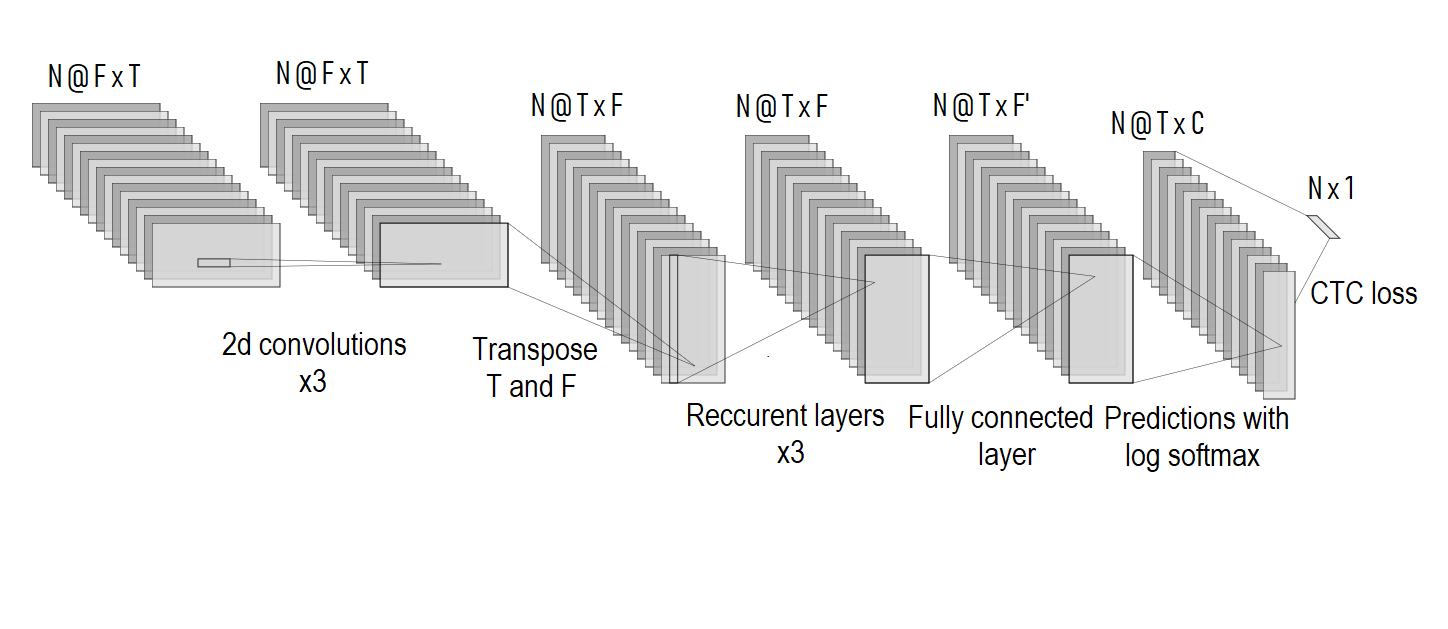
\includegraphics[width=\textwidth]{net_model.png}
		\captionsetup{justification=centering}
		\caption{Model of the network. F -- number of frequency bins, F'~--~number of frequency bins after linear map,  T~--~number of time frames, C~--~size of the alphabet}
		\label{fig:arch}
	\end{figure}
	
	Softmax function $f : \mathbb{R}^k \rightarrow \mathbb{R}^k$ is defined by the formula:
	$$
	f_i(v) = \frac{e^{v_i}}{\sum_{i=1}^{k} e^{v_j}},
	$$
	and
	$$
	f(v) = \big(f_1(v), f_2(v), \ldots, f_k(v) \big).
	$$
	We apply exponential function to each outputted value, and then normalize these values to make sure that probabilities sum up to 1. In our case $k=29$, hence there is 29 possible output characters to distribute probability on (26 letters and 3 special symbols, as described in section \ref{sec:input}).
	
	\section{CTC Loss} \label{sec:ctc}
	To train a neural network, we typically need a function that would tell us how good current network's output is. The lesser value this function has, the better results our model achieves. This kind of function is called a \textbf{loss function}. Usually, minimizing a value of the loss function is a main goal of the training.
	
	Loss function used in DS2 is \textbf{Connectionist Temporal Classification} (CTC) \cite{DS3}. To define this loss, let us introduce an encoding of a text. Encoding of a given text \textit{S} is done by replacing every character \textit{c} in \textit{S} by any number of characters \textit{c} and blanks "-". The only restriction is that if there are two adjacent identical letters in \textit{S}, they must be separated by a blank "-".
	
	For instance, possible encodings of \textit{"to"} are \textit{"-tttooo"} and \textit{"-tttoo-o"}, but only the latter could be an encoding of the word \textit{"too"}.
	
	Now we say that the probability of an actual transcription is the sum of probabilities of all possible encodings of the actual transcription, that have the same length as the output of the model. The loss function here is simply the negative logarithm of this probability. Having this we can count derivatives of this loss function with respect to model output and then apply \textit{backpropagation through time} algorithm to train the network, which is just a standard backpropagation algorithm modified for recurrent neural networks.
	
	\section{Training} \label{sec:trainig}
	During training, datasets are divided into batches of some certain size. Batches are fed one by one into the model and after each one CTC loss is computed and backpropagated through the network, and then weights on the layers are updated. The speed in which changes are applied to the model depends on some chosen parameter -- \textbf{learning rate}. All batches make up for an epoch of training and training lasts for many epochs -- until loss does not decrease anymore or decreases very slightly.
	Accuracy of the model is measured by \textbf{Word Error Rate} (WER) \cite{DS1}. It is a common metric of the performance of speech recognition systems. Many commercial ASR systems are beeing compared using WER \cite{DS8}. To measure Word Error Rate, we compare the recognized word sequence with a reference word sequence by transforming the latter to the former and find:
	
	\begin{itemize}
		\item $S$ -- the number of substitutions,
		\item $D$ -- the number of deletions,
		\item $I$ -- the number of insertions,
		\item $C$ -- the number of correct words,
		\item $N$ -- the number of words in the reference ($N=S+D+C$).
	\end{itemize}
	Now the WER can be computed as:
	$$
	\text{WER} = \frac{S + D + I}{N} = \frac{S + D + I}{S + D + C}.
	$$
	
	\section{Generating transcription} \label{sec:transcription}
	In order to find Word Error Rate of the model, one has to generate some final transcription. It is generated based on both output of the model and an $N$-gram language model \cite{DS9}. To generate the final transcription, we search for transcription \textit{y} that maximizes \textit{Q(y)}, where \textit{Q} is given as follows:
	$$
	Q(y) = \log \big(\mathbb{P}_{ctc}(y|x)\big) + \alpha \cdot \log \big( \mathbb{P}_{lm}(y) \big) + \beta \cdot \text{word\_count}(y).
	$$
	The term $\mathbb{P}_{ctc}(y|x)$ denotes the probability of $y$ being a transcription of the utterance $x$ as described in section 1.3 and the term $\mathbb{P}_{lm}(y)$ denotes the probability of the sequence $y$ according to the language model. The weights $\alpha$ and $\beta$ are tunable parameters and control the contribution of the language model and word count in scoring of transcription. We use a beam search similar to one described in \cite{DS7} to find the optimal transcription \textit{y}.
	
	Beam search is an algorithm that iterates over each time-step in the output of DS2 model, while remembering some constant number (let this number be $BW$ -- \textit{Beam Width}) of the most probable transcriptions up to this point. When considering the next time-step, we create $BW \cdot C$ new transcriptions corresponding to appending every possible character (we denote number of them by $C$) to the end of each of $BW$ remembered transcriptions. After merging identical transcriptions and recalculating their probabilities we again keep $BW$ best ones. In the end we have $BW$ \textit{most probable} transcriptions, so we just take the best one.
	
	In order to efficiently merge transcriptions and recalculate new probabilities for them, we must store probabilities $\mathcal{P}_{b}$, $\mathcal{P}_{nb}$, $\mathcal{P}_{lm}$ for all kept transcriptions, where:
	\begin{itemize}
		\item $\mathcal{P}_{b}(y, t)$ -- probability of the given transcription $y$ at time-step $t$ if the encoding ends with \textit{blank},
		\item $\mathcal{P}_{nb}(y, t)$ -- probability of the given transcription $y$ at time-step $t$ if the encoding doesn't end with \textit{blank},
		\item $\mathcal{P}_{lm}(y)$ -- probability of the given transcription $y$, according to the language model.\\
	\end{itemize}
	
	\section{Summary}
	To sum up, workflow in DS2 is typical for neural networks. We prepare some data in the form described in section \ref{sec:input}. Next we forward propagate the data through the layers described in section \ref{sec:layers}. After that we count CTC Loss (section \ref{sec:ctc}) and update model weights with specific learning rate (section \ref{sec:trainig}). To evaluate the model we generate transcription from predictions given by the output layer using beam search algorithm (section \ref{sec:transcription}) and count Word Error Rate metrics (section \ref{sec:trainig}).
	
	
	\chapter{Implemented features and results}\label{r:results}
    
    
    
    
    
    
    
    
    
    
    
    	\section{Mixed precision training}
	In order to speed up training, we decided to try to reduce precision of floating-point calculations, where full precision is not really needed to achieve comparable accuracy.
	
	Standard deep learning frameworks, such as PyTorch, use 32 bit floating point variables (FP32) to keep model parameters, and perform all operations. Massively parallel architecture of modern GPUs allows to perform in the same time much more arithmetic operations on 16 bit floating-point variables (FP16) than on 32 bit variables.
	Specifically, performance can be boosted by using Tensor Cores: hardware units prepared to accelerate matrix multiplications, introduced by Nvidia in Volta GPU architecture \cite{MPT}.
	So reducing precision could not only reduce memory consumption but also measurably improve time needed for model convergence.
	
	A common technique, used to improve speed, but not to break performance, is to keep model weights in two copies -- one in FP32 and one in FP16. In each iteration we would use FP16 one to perform forward, backward propagation, and then to calculate gradients of every weight. Then we would use these gradients to update weights of original, FP32 model weights. Finally, we would make a new instance of FP16 model weight by cutting off precision of updated FP32 model \cite{APEX}.
	
	Another heuristic is to split operations on tensors into two groups. In the first group we would place, for instance, transitions through fully connected and convolutional layers, in general, computational heavy and precision safe operations. In the second group we would place all the other operations: for instance softmax and batchnorm. Now we would port operations from the first group to FP16 and keep operations from the second group in FP32. This way we would be safe from precision issues and still achieve pretty good speedup (in comparison to the model, that performs all computations in FP16) \cite{APEX}.
	
	There is one more thing, we need to care about, while reducing precision. FP16 uses only 5 bits for exponent, and its representable range is quite narrow, so that in some cases gradients are small enough to be eventually rounded to 0. To prevent that, one may multiply loss by a power of two, then perform backward propagation algorithm, and then scale back obtained gradients. This solution works well in practice. However now we have to deal with another problem. Gradients calculated in the process may overflow. And even one overflow unables us to calculate gradients for parameters depended on that particular weight. So the scaling factor, rather than being one fixed power of two, need to be adjusted during training: decreased after detection of overflow and increased if too many gradients are zeroed as a result of rounding \cite{LOSS_SCALING}.
	
	Speaking from more practical side, we used Apex AMP, which is a PyTorch extension developed to ease mixed precision training. It supports automatic dynamic loss scaling, and both described above ways of performing mixed precision training. Further description of this tool can be found in \cite{APEX_DOCS}.
	
	
	\begin{figure}[!hbt]
		\begin{center}
			\begin{tikzpicture}
			\begin{axis}[
			ymin = 0, ymax = 1,
			xmin = 0, xmax = 13,
			minor y tick num = 4,
			minor x tick num = 1,
			ymajorgrids = true,
			grid style = dashed,
			%area style,
			scaled x ticks = false,
			xlabel = Epochs,
			ylabel = CTCLoss,
			legend pos=outer north east,
			no markers            
			]
			\addplot[dashed, color=blue] table[x=epochs,y=training]{\amp};
			\addlegendentry{Training MP}
			\addplot[ color=blue] table[x=epochs,y=validation]{\amp};
			\addlegendentry{Validation MP}
			\addplot[dashed, color=red] table[x=epochs,y=training]{\norm};
			\addlegendentry{Training FP$32$}
			\addplot[color=red] table[x=epochs,y=validation]{\norm};
			\addlegendentry{Validation FP$32$}
			\end{axis}
			\end{tikzpicture}
		\end{center}
		\caption{Comparison of training with and without AMP.}
		\label{fig:amp}
	\end{figure}
	
	Figure \ref{fig:amp} presents comparison of training process with and without AMP, denoted as MP (standing for Mixed Precision) and FP32 respectively. We used the same architecture and the same hyperparameters in both cases. One epoch in FP32 lasted for around $135$ minutes, while in mixed precision only $75$ minutes. Therefore, we got $1.8$ speedup. When it comes to the performance, one can see from the figure \ref{fig:amp} that the training loss was falling more or less in the same way. To measure models performance we calculated the validation loss -- loss function on all examples from the validation dataset. The reason for this is that computing the validation loss is less computationally expensive then WER. We found that validation loss was always a bit lower for FP32 training. Figure \ref{fig:wer} shows that FP32 model was a bit better also in WER as final WER for FP32 was $13.1$\% and for MP it was $13.84$\%. Looking at validation loss, we can conclude, that we can use it as a convenient metric to know when we should stop trainig and we can calculate loss function only after training is finished. What's more, we decided to run rest of experiments only with AMP as it gives us comparable results as usual FP32 training and is much faster.
	
	
	\pgfplotstableread[row sep=\\,col sep=&]{
		epochs & amp & noamp \\ 
		2 & 0.251 & 0.19 \\
		4 & 0.2 & 0.163 \\
		6 & 0.181 & 0.156 \\
		8 & 0.164 & 0.136 \\
		10 & 0.159 & 0.131 \\
		12 & 0.144 & 0.131 \\
	}\wercomp
	
	\begin{figure}[!hbt]
		\begin{center}
			\begin{tikzpicture}
			\begin{axis}[
			ymin = 0, ymax = 0.4,
			xmin = 2, xmax = 12,
			minor y tick num = 4,
			minor x tick num = 1,
			ymajorgrids = true,
			grid style = dashed,
			%area style,
			scaled x ticks = false,
			xlabel = Epochs,
			ylabel = WER,
			legend pos=outer north east,
			no markers            
			]
			\addplot[color=blue] table[x=epochs,y=amp]{\wercomp};
			\addlegendentry{MP}
			\addplot[color=red] table[x=epochs,y=noamp]{\wercomp};
			\addlegendentry{FP$32$}
			\end{axis}
			\end{tikzpicture}
		\end{center}
		\caption{Comparison of WER with and without AMP.}
		\label{fig:wer}
	\end{figure}
    
    
    	\section{Language model and decoding predictions}
	\textbf{$N$-gram language model} is a model of a language in which we assign probabilities of occurrence to sequences of N words based on some large unlabelled text data. Incorporating model to prediction decoding helps avoid typos which are usually phonetically plausible and often occur on words that rarely or never occur in training set. We use Librispeech 4-gram language model available in \cite{LM-LINK}.
	
	Performances with the language model in comparison to no language model are $13.84$\% WER and $14.22$\% WER.
	
	At the beginning we also experimented with an easier language model that assigned probabilities to sequences of letters as it was much smaller and simpler. Unfortunately WER was increasing after applying such LM so we abandoned this idea for the bigger and more reliable N-gram LM.
	
	
    	\section{Performance and multi GPU scaling}
	For training, we used machine with Intel(R) Xeon(R) CPU E5-2698 v4 @ 2.20GHz, (which has 20 physical cores), and 256 GB of RAM. It was equipped with four Nvidia Tesla V100 GPUs (32 GB of global memory each), connected by NVlink.
	
	Table \ref{tab:multi} describes performance and scaling we achieved by utilizing more than one GPUs. We measured time that took training for one epoch on full dataset of 960 hours.
	
	{
		\centering
		\begin{tabular}{|c|c|c|}
			\hline
			number of GPUs & time in minutes & speedup \\
			\hline
			1 GPU & 119 & 1 \\
			\hline
			2 GPUs & 75 & 1.57 \\
			\hline
			4 GPUs & 35 & 3.37 \\
			\hline
		\end{tabular}
		\label{tab:multi}
		\captionof{table}{Epoch training time comparison}
	}
	
	For $11$ epochs long mixed precision training on 4 GPUs standard deviation of an epoch time was approximately $14$ seconds. It shows that network is scalable, and can be extended to more GPUs.
    
    
    \section{Training dataset}
	As our dataset we use ''LibriSpeech ASR corpus'' \cite{DATA} -- public ASR dataset containing 960 hours of audiobook English speech for training together with test datasets. This dataset is much smaller than the dataset used in original Deep Speech 2 paper. Unfortunately original Deep Speech 2 dataset is not publicly available and almost impossible to reproduce with limited resources. However, many other works rely on Librispeech as their dataset \cite{LIBRI-EX}.
	
	We report our results on model trained on 460 hours of ''clean'' speech and 960 hours of combined 460 hours of ''clean'' speech and 500 hours of ''other'' speech in figure \ref{fig:dataset}.
	
	\pgfplotstableread[row sep=\\,col sep=&]{
		epochs & training & validation \\ 
		1 & 1.78 & 0.87 \\
		2 & 0.70 & 0.56 \\
		3 & 0.48 & 0.47 \\
		4 & 0.36 & 0.41 \\
		5 & 0.29 & 0.39 \\
		6 & 0.24 & 0.33 \\
		7 & 0.21 & 0.31 \\
		8 & 0.18 & 0.34 \\
		9 & 0.15 & 0.34 \\
		10 & 0.13 & 0.31 \\
		11 & 0.12 & 0.34 \\
		12 & 0.10 & 0.32 \\
		13 & 0.09 & 0.34 \\
		14 & 0.08 & 0.36 \\
		15 & 0.07 & 0.37 \\
		16 & 0.07 & 0.37 \\
		17 & 0.06 & 0.40 \\
		18 & 0.06 & 0.34 \\
		19 & 0.05 & 0.40 \\
	}\clean
	
	\noindent%
	\begin{minipage}{\linewidth}% to keep image and caption on one page
		\makebox[\linewidth]{%        to center the image
			\begin{tikzpicture}
			\begin{axis}[
			ymin = 0, ymax = 2,
			xmin = 0, xmax = 13,
			minor y tick num = 4,
			minor x tick num = 1,
			ymajorgrids = true,
			grid style = dashed,
			scaled x ticks = false,
			xlabel = Epochs,
			ylabel = CTC Loss,
			legend pos=outer north east,
			no markers
			]
			\addplot[dashed, color=red] table[x=epochs,y=training]{\clean};
			\addlegendentry{training with clean dataset}		  
			\addplot[color=red] table[x=epochs,y=validation]{\clean};
			\addlegendentry{validation with clean dataset}
			\addplot[dashed, color=blue] table[x=epochs,y=training]{\amp};
			\addlegendentry{training with mixed dataset}		  
			\addplot[color=blue] table[x=epochs,y=validation]{\amp};
			\addlegendentry{validation with mixed dataset}
			
			\end{axis}
			\end{tikzpicture}
		}\captionof{figure}{Dataset type plot}
		\label{fig:dataset}		     
	\end{minipage}\\
	
	WER of model trained on 460 hours dataset is $23.35$\% and WER of the one trained on 960 hours $13.84$\%.
	
	
	\chapter{Experiments on architecture and hyperparameters}\label{r:experiments}

	
	\section{Recurrent unit type}
	\pgfplotstableread[row sep=\\,col sep=&]{
		epochs & training & validation \\ 
		1 & 1.34 & 0.59 \\
		2 & 0.57 & 0.38 \\
		3 & 0.41 & 0.28 \\
		4 & 0.32 & 0.27 \\
		5 & 0.27 & 0.25 \\
		6 & 0.23 & 0.25 \\
		7 & 0.20 & 0.25 \\
		8 & 0.17 & 0.25 \\
		9 & 0.15 & 0.21 \\
		10 & 0.13 & 0.26 \\
		11 & 0.12 & 0.22 \\
		12 & 0.11 & 0.26 \\
	}\rnn
	
	\pgfplotstableread[row sep=\\,col sep=&]{
		epochs & training & validation \\ 
		1 & 1.58 & 0.59 \\
		2 & 0.54 & 0.35 \\
		3 & 0.35 & 0.29 \\
		4 & 0.25 & 0.25 \\
		5 & 0.19 & 0.26 \\
		6 & 0.15 & 0.26 \\
		7 & 0.12 & 0.25 \\
		8 & 0.10 & 0.25 \\
		9 & 0.09 & 0.27 \\
		10 & 0.08 & 0.25 \\
		11 & 0.07 & 0.27 \\
		12 & 0.06 & 0.27 \\
		13 & 0.05 & 0.32 \\
		14 & 0.05 & 0.26 \\
		15 & 0.05 & 0.31 \\
		16 & 0.04 & 0.33 \\
		17 & 0.04 & 0.33 \\
		18 & 0.04 & 0.35 \\
		19 & 0.04 & 0.30 \\
		20 & 0.03 & 0.30 \\
		21 & 0.03 & 0.30 \\
	}\gru
	
	\pgfplotstableread[row sep=\\,col sep=&]{
		epochs & training & validation \\ 
		1 & 1.14 & 0.39 \\
		2 & 0.37 & 0.25 \\
		3 & 0.23 & 0.21 \\
		4 & 0.16 & 0.20 \\
		5 & 0.11 & 0.18 \\
		6 & 0.08 & 0.19 \\
		7 & 0.06 & 0.21 \\
		8 & 0.05 & 0.22 \\
		9 & 0.04 & 0.23 \\
		10 & 0.03 & 0.23 \\
		11 & 0.03 & 0.22 \\
		12 & 0.03 & 0.24 \\
		13 & 0.02 & 0.27 \\
		14 & 0.02 & 0.25 \\
		15 & 0.02 & 0.27 \\
		16 & 0.02 & 0.26 \\
		17 & 0.01 & 0.27 \\
	}\lstm
	
	In section \ref{sec:layers} we mentioned bidirectional recurrent layers. Three most commonly used ones are vanilla \textbf{Recurrent Neural Networks} (RNN) \cite{RNN}, \textbf{Long Short Term Memory Unit} (LSTM) \cite{LSTM} and \textbf{Gated Recurrent Unit} (GRU) \cite{GRU}. We will deliver a brief description of these units based on \cite{DS2}.
	
	Let's denote by $l$ the layer number. A bidirectional recurrent layer $h^l$ consists of a forward recurrent layer $\overrightarrow{h^l}$ and a backward recurrent layer $\overleftarrow{h^l}$. The forward and backward recurrent layer activations for time $t$ are computed as $\overrightarrow{h^l_t} = g(\overrightarrow{h^l_{t - 1}}, h^{l-1}_t)$ and $\overleftarrow{h^l_t} = g(\overleftarrow{h^l_{t+1}}, h^{l-1}_t)$. In the end, we add both partial layers to get $h^l = \overrightarrow{h^l} + \overleftarrow{h^l}$.
	
	Function $g$ mentioned before depends on specific recurrent unit type. For vanilla RNN it is just
	$$\overrightarrow{h^l_t} = f\big(W^l h^{l-1}_t + \overrightarrow{U^l} \overrightarrow{h^l_{t - 1}} + b^l\big)$$
	and similarly for the backward recurrent layer. Here $W^l$ and $\overrightarrow{U^l}$ are just weight matrices, $b^l$ is a bias vector and $f$ is an activation function (e.g. ReLU or tanh). For LSTM and GRU function $g$ is much more complex.
	
	\noindent%
	\begin{minipage}{\linewidth}% to keep image and caption on one page
		\makebox[\linewidth]{%        to center the image
			\begin{tikzpicture}
			\begin{axis}[
			ymin = 0, ymax = 1.75,
			xmin = 0, xmax = 12,
			minor y tick num = 4,
			minor x tick num = 0,
			ymajorgrids = true,
			grid style = dashed,
			scaled x ticks = false,
			xlabel = Epochs,
			ylabel = CTC Loss,
			legend pos=outer north east,
			no markers
			]
			\addplot[dashed, color=red] table[x=epochs,y=training]{\gru};
			\addlegendentry{training with GRU}		  
			\addplot[color=red] table[x=epochs,y=validation]{\gru};
			\addlegendentry{validation with GRU}
			\addplot[dashed, color=blue] table[x=epochs,y=training]{\rnn };
			\addlegendentry{training with RNN}		  
			\addplot[color=blue] table[x=epochs,y=validation]{\rnn};
			\addlegendentry{validation with RNN}
			
			
			
			\end{axis}
			\end{tikzpicture}
		}\captionof{figure}{RNN vs GRU plot}
		\label{fig:gru}		     
	\end{minipage}
	
	\noindent
	As we can see in figure \ref{fig:gru} there is a noticeable difference in training loss of GRU and RNN layers. In fact, GRU layer achieved WER of $14.66$\% while RNN layer achieved $13.84$\%.
	\\
	
	\noindent%
	\begin{minipage}{\linewidth}% to keep image and caption on one page
		\makebox[\linewidth]{%        to center the image
			\begin{tikzpicture}
			\begin{axis}[
			ymin = 0, ymax = 1.5,
			xmin = 0, xmax = 12,
			minor y tick num = 4,
			minor x tick num = 1,
			ymajorgrids = true,
			grid style = dashed,
			scaled x ticks = false,
			xlabel = Epochs,
			ylabel = CTC Loss,
			legend pos=outer north east,
			no markers
			]
			\addplot[dashed, color=red] table[x=epochs,y=training]{\lstm};
			\addlegendentry{training with LSTM}		  
			\addplot[color=red] table[x=epochs,y=validation]{\lstm};
			\addlegendentry{validation with LSTM}
			\addplot[dashed, color=blue] table[x=epochs,y=training]{\rnn };
			\addlegendentry{training with RNN}		  
			\addplot[color=blue] table[x=epochs,y=validation]{\rnn};
			\addlegendentry{validation with RNN}
			
			
			
			\end{axis}
			\end{tikzpicture}
		}\captionof{figure}{RNN vs LSTM plot}
		\label{fig:lstm}		     
	\end{minipage}
	
	Validation loss with LSTM layer appeared to converge faster than validation loss with RNN layer. In fact, it achieved better WER. Nevertheless we decided to use vanilla RNN in our experiments as it's faster -- it is shown in table \ref{tab:rec}.
	
	{
		\centering
		\begin{tabular}{|c|c|c|}
			\hline
			RNN & GRU & LSTM \\
			\hline
			\hline
			35 & 53 & 43 \\
			\hline
		\end{tabular}
		\captionof{table}{Epoch training time in minutes}
		\label{tab:rec}
	}
	
	WER results with GRU and LSTM are $14.66$\% and $11.57$\% respectively compared to $13.84$\% of vanilla RNN.
	

	\section{Regularization}
	\subsection{Batch normalization}
	Batch normalization is a technique for improving the speed, performance, and stability of artificial neural networks, primarily introduced to reduce internal covariate shift \cite{BN}. Method based on the idea of normalizing data within each mini-batch using stochastic optimizations for mean and variance.
	
	Denote by $B$ mini-batch of a training set, by $m$ size of $B$. If input is $d$--dimensional: $x = (x^{(1)}, x^{(2)}, \ldots, x^{(d)})$, we calculate mean and variance as follows:
	$$\mu^{(k)} = \frac{1}{m}\sum_{i=1}^m x^{(k)}_i$$
	
	$$ \sigma^{{(k)}^2} = \frac{1}{m-1} \sum_{i = 1}^{m} \left(x^{(k)}_i - \mu^{(k)}\right) ^ 2.$$
	Next step is normalization:
	
	$$
	\hat{x} ^ {(k)} _ i = \frac{x^{(k)}_i - \mu^{(k)}} {\sqrt{ \sigma^{{(k)}^2} + \epsilon}}
	$$
	where $\epsilon$ is small constant added for numerical stability. Finally we scale and shift normalized data:
	
	$$ y^{(k)}_i = \gamma^{(k)} \hat{x}^{(k)}_i + \beta^{(k)}$$
	where $\gamma^{(k)}$ and $\beta^{(k)}$ are learnable parameters.
	
	In our model we use batch normalization after each convolutional layer. When we tried training our model without batch normalization layers, we found out that model didn't learn. Training loss was very high, over $2.5$, and validation loss was NaN. That experiment clearly shows that batch normalization is crucial for proper model training and without it we can't expect model to work correctly.
	
	\subsection{Dropout}
	Dropout is regularization strategy patented by Google \cite{DROPG}, it is used to remove neural network overfitting. The basic idea of this technique consists in multiplying input and hidden units, during training process, by randomly generated bit mask (or in other words with a given probability we decide whether or not given neuron will be used in the next iteration) \cite{DROPW}. It follows that some nodes will be inactive, set to 0, and model is prevented from complex co-adaptations.
	
	\pgfplotstableread[row sep=\\,col sep=&]{
		epochs & training & validation \\ 
		1 & 2.02 & 0.76 \\
		2 & 0.66 & 0.44 \\
		3 & 0.45 & 0.33 \\
		4 & 0.35 & 0.28 \\
		5 & 0.29 & 0.27 \\
		6 & 0.24 & 0.25 \\
		7 & 0.21 & 0.24 \\
		8 & 0.18 & 0.23 \\
		9 & 0.16 & 0.24 \\
		10 & 0.14 & 0.23 \\
		11 & 0.12 & 0.23 \\
		12 & 0.11 & 0.24 \\
		13 & 0.10 & 0.25 \\
		14 & 0.09 & 0.25 \\
		15 & 0.08 & 0.26 \\
		16 & 0.07 & 0.26 \\
		17 & 0.07 & 0.26 \\
		18 & 0.06 & 0.27 \\
	}\dropouticm
	
	
	
	\noindent%
	\begin{minipage}{\linewidth}% to keep image and caption on one page
		\makebox[\linewidth]{%        to center the image
			\begin{tikzpicture}
			\begin{axis}[
			ymin = 0, ymax = 2,
			xmin = 0, xmax = 13,
			minor y tick num = 4,
			minor x tick num = 1,
			ymajorgrids = true,
			grid style = dashed,
			scaled x ticks = false,
			xlabel = Epochs,
			ylabel = CTC Loss,
			legend pos=outer north east,
			no markers
			]
			\addplot[dashed, color=red] table[x=epochs,y=training]{\dropouticm};
			\addlegendentry{training without dropout}
			\addplot[color=red] table[x=epochs,y=validation]{\dropouticm};
			\addlegendentry{validation without dropout}
			\addplot[dashed, color=blue] table[x=epochs,y=training]{\amp};
			\addlegendentry{normal training}		  
			\addplot[color=blue] table[x=epochs,y=validation]{\amp};
			\addlegendentry{normal validation}
			
			
			
			\end{axis}
			\end{tikzpicture}
		}\captionof{figure}{Dropout plot}
		\label{fig:dropout}		     
	\end{minipage}
	
	Figure \ref{fig:dropout} presents results of our experiments with and without dropout. One can see that dropout has the biggest impact in the beginning of the training but as the time goes by, results of both versions are getting similar. However, even after longer training WER results differ: $13.84$\% for net with dropout and $16.48$\% for net without dropout.
	
	
	\subsection{L2 regularization}
	$L2$ regularization is a technique designed to prevent neural network from overfitting training dataset. The key idea behind this method consists in keeping network weights from growing too large unless it is really necessary. It can be realized by adding a term $\lambda ||W||^2_F $ to the cost function that penalizes large weights, where $||W||_F $ is
	a Frobenius norm, and $\lambda$ is parameter governing how strongly large weights are penalized \cite{L2}.
	
	Performed experiments showed that applying L2 regularization does not have positive effect on loss function convergence. With weight decay scale equal to $0.0005$ CTC loss oscillated around $1$.
	
	
	

	
	
	\section{Sortagrad and dataset sorting}
	Training examples that we use vary in length. Longer examples may be described as more challenging. Additionally, as CTC cost function is a negative logarithm of probability, it gets bigger for longer utterances. Authors of Deep Speech 2 also suspect that these longer utterances usually have bigger gradients. Their proposition for challenging varying length of examples is \textbf{SortaGrad}. Instead of training on minibatches in random order, in the first epoch we sort them in the increasing order of longest utterance of minibatch. From the second epoch they are shuffled again.
	
	Unfortunately, Apex AMP only supports shuffling dataset for distributed training. Therefore we were not able to test, how sortagrad would affect our results.
	
	\pgfplotstableread[row sep=\\,col sep=&]{
		epochs & training & validation \\ 
		1 & 1.53 & 0.66 \\
		2 & 0.62 & 0.40 \\
		3 & 0.44 & 0.31 \\
		4 & 0.35 & 0.27 \\
		5 & 0.29 & 0.26 \\
		6 & 0.25 & 0.24 \\
		7 & 0.21 & 0.23 \\
		8 & 0.19 & 0.23 \\
		9 & 0.16 & 0.22 \\
		10 & 0.15 & 0.23 \\
		11 & 0.13 & 0.24 \\
		12 & 0.12 & 0.24 \\
		13 & 0.11 & 0.24 \\
		14 & 0.10 & 0.23 \\
		15 & 0.09 & 0.24 \\
		16 & 0.08 & 0.25 \\
		17 & 0.08 & 0.26 \\
		18 & 0.07 & 0.26 \\
	}\xavier
	
	\section{Xavier initialization}
	We use Xavier initialization \cite{XAVIER} for weights in our model. It is a heuristic random initialization of trainable weights in a neural network that assigns values sampled from normal distribution $$\mathcal{N}\left(0, \sqrt{\frac{2}{N_{in} + N_{out}}}\right)$$ where $N_{in}$ is number of inputs and $N_{out}$ is number of outputs of a certain layer. Parameters of the distribution are chosen in such a way that variances of input to Xavier -- intialized layer and output of that layer differ slightly. This prevents exploding and diminishing values during both forward and backward pass through the network and thus speeds up learning.
	
	\noindent%
	\begin{minipage}{\linewidth}% to keep image and caption on one page
		\makebox[\linewidth]{%        to center the image
			\begin{tikzpicture}
			\begin{axis}[
			ymin = 0, ymax = 2,
			xmin = 0, xmax = 13,
			minor y tick num = 4,
			minor x tick num = 1,
			ymajorgrids = true,
			grid style = dashed,
			scaled x ticks = false,
			xlabel = Epochs,
			ylabel = CTC Loss,
			legend pos=outer north east,
			no markers
			]
			\addplot[dashed, color=red] table[x=epochs,y=training]{\xavier};
			\addlegendentry{training with default initialization}		  
			\addplot[color=red] table[x=epochs,y=validation]{\xavier};
			\addlegendentry{validation with default initialization}
			\addplot[dashed, color=blue] table[x=epochs,y=training]{\amp};
			\addlegendentry{training with Xavier initialization}		  
			\addplot[color=blue] table[x=epochs,y=validation]{\amp};
			\addlegendentry{validation with Xavier initialization}
			
			\end{axis}
			\end{tikzpicture}
		}\captionof{figure}{Xavier initialization plot}
		\label{fig:xavier}		     
	\end{minipage}\\
	
	
	One can easily see in figure \ref{fig:xavier} that Xavier initialization outperforms default PyTorch initialization in the early stage of training. After around 10 epochs both models have more or less the same training and validation loss -- it means that when we train model for a longer time benefits of a proper initialization are not so important. Final WER in both cases is $13.84$\% and $15.24$\% for model with Xavier initialization and no initialization respectively.
	
	
	
	\section{Hyperparameters}
	To achieve the best accuracy and performance we had to determine what should be values of hyperparameters (e.g. learning rate, batch size, convolutional kernel size, number of features in fully connected layer etc.). We did it by training our network many times with various combinations of mentioned hyperparameters. We looked at results and, according to our intuitions, tried to modify them to achieve better accuracy. What we present in final training scripts is the best combination we found. Probably, there are better ones, but what we have allows us to train model and achieve state of the art accuracy.
	
	
	\chapter{Conclusions}\label{r:concls}
	
	To sum up, we present PyTorch scripts for training Deep Speech 2 model for ASR. We also provide already trained models as well as the results of our experiments justifying using specific architecture solutions.
	
	The best model we managed to train achieved $11.57$\% WER after training for 9 hours. One should notice that original Deep Speech 2 model trained on 1200 h dataset achieved $13.8$\% WER \cite{DS2}, but it used dataset with conversations as well as monologues (and we used monologues only) -- that probably explains our better performance. Nevertheless, we can state that we managed to implement and train state of the art model for ASR.
	
	We also managed to speed-up training using potential of GPUs -- we trained our model in mixed precision and used multiple GPUs for it. We also showed how exactly that optimizations speed-up training process.
	
	In the future we plan to use prepared model for recognizing other languages. The main problem is finding appropriate datasets -- we want ones that are free and have sufficiently short utterances. If we cannot find such dataset we can try generating it on our own (e.g. splitting audio-books into shorter parts). We assume that probably we will have to change some hyperparameters but the core architecture should stay the same.
	
	\appendix
	
	\chapter{}
	
	We attach a DVD containing: 
	
	\begin{itemize}
		\item this paper as both pdf file and tex source file,
		\item presentation,
		\item poster,
		\item two pretrained models, which are the best in metric of achieved WER -- one trained in FP32 and one trained in mixed precision.
	\end{itemize}
	
	\begin{thebibliography}{99}
		\addcontentsline{toc}{chapter}{Bibliography}
		
		\bibitem{L2} Anders Krogh, John A. Hertz, \textit{A Simple Weight Decay Can Improve Generalization}, \href{https://papers.nips.cc/paper/563-a-simple-weight-decay-can-improve-generalization.pdf}{https://papers.nips.cc/paper/563-a-simple-weight-decay-can-improve-generalization.pdf}
		
		\bibitem{DROPW} David Warde-Farley, Ian J. Goodfellow, Aaron Courville, Yoshua Bengio, \textit{An empirical analysis of dropout in piecewise linear networks},  \href{https://arxiv.org/abs/1312.6197}{https://arxiv.org/abs/1312.6197}
		
		\bibitem{BN} Sergey Ioffe, Christian Szegedy, \textit{Batch Normalization: Accelerating Deep Network Training by Reducing Internal Covariate Shift},  \href{https://arxiv.org/pdf/1502.03167.pdf}{https://arxiv.org/pdf/1502.03167.pdf}
		
		\bibitem{RNN} M. Schuster \& K. K. Paliwal, \textit{Bidirectional recurrent neural networks}, IEEE Transactions on Signal Processing, 45(11):2673–2681, 1997,  \href{https://pdfs.semanticscholar.org/4b80/89bc9b49f84de43acc2eb8900035f7d492b2.pdf}{https://pdfs.semanticscholar.org/4b80/89bc9b49f84de43acc2eb8900035f7d492b2.pdf}
		
		\bibitem{DS8} Bohouta, Gamal \& Këpuska, Veton, \textit{Comparing Speech Recognition Systems (Microsoft API, Google API And CMU Sphinx)}, Int. Journal of Engineering Research and Application, 2248-9622, 20-24, 10.9790/9622-0703022024
		
		\bibitem{DS3} A. Graves, S. Fernandez, F. Gomez, and J. Schmidhuber, \textit{Connectionist temporal classification:
			Labelling unsegmented sequence data with recurrent neural networks}, in ICML, pages 369-376, ACM, 2006
		
		\bibitem{DS1} Hannun et al,
		\textit{Deep Speech: Scaling up end-to-end speech recognition}, Silicon Valley AI Lab 2014, \href{https://arxiv.org/abs/1412.5567}{https://arxiv.org/abs/1412.5567}
		
		\bibitem{DS2} Baidu Research, \textit{Deep Speech 2: End-to-End Speech Recognition in English and Mandarin}, Silicon Valley AI Lab 2015, \href{https://arxiv.org/abs/1512.02595}{https://arxiv.org/abs/1512.02595}
		
		\bibitem{DS7} A. Y. Hannun, A. L. Maas, D. Jurafsky, and A. Y. Ng, \textit{First-pass large vocabulary continuous speech recognition using bi-directional recurrent DNNs}, \href{http://arxiv.org/abs/1408.2873}{http://arxiv.org/abs/1408.2873}
		
		\bibitem{LIBRI-EX} Jayadev Billa, \textit{Improving LSTM-CTC based ASR performance in domains with limited training data}, 
		\href{https://arxiv.org/pdf/1707.00722.pdf}{https://arxiv.org/pdf/1707.00722.pdf}
		
		\bibitem{LIBRI} Vassil Panayotov, Guoguo Chen, Daniel Povey and Sanjeev Khudanpur, \textit{LibriSpeech: an ASR corpus based on public domain audio books}, 
		\href{http://www.openslr.org/12/}{http://www.openslr.org/12/}
		
		\bibitem{DATA} LibriSpeech ASR corpus,  \href{http://www.openslr.org/12/}{http://www.openslr.org/12/}
		
		\bibitem{LM-LINK} Librispeech language model,
		\href{http://www.openslr.org/resources/11/}{http://www.openslr.org/resources/11/}
		
		\bibitem{LSTM} S. Hochreiter \& J. Schmidhuber, \textit{Long short-term memory}, Neural Computation 9(8):1735—1780, 1997,  \href{https://www.bioinf.jku.at/publications/older/2604.pdf}{https://www.bioinf.jku.at/publications/older/2604.pdf}
		
		\bibitem{MPT}  P. Micikevicius, S. Narang, J. Alben, G. Diamos, E. Eelsen, B. Ginsburg, M. Houston, O. Kuchaiev, G. Venkatesh, H. Wu, \textit{Mixed Precision Training},
		\href{https://arxiv.org/abs/1710.03740}{https://arxiv.org/abs/1710.03740}
		
		\bibitem{DS9} Daniel Jurafsky \& James H. Martin, \textit{N-gram Language Models}, 	\href{https://web.stanford.edu/~jurafsky/slp3/3.pdf}{https://web.stanford.edu/~jurafsky/slp3/3.pdf}
		
		\bibitem{APEX_DOCS}
		NVIDIA Apex documentation,
		\href{https://nvidia.github.io/apex/amp.html}{https://nvidia.github.io/apex/amp.html}
		
		
		\bibitem{APEX}
		Carl Case, Michael Carilli, \textit{NVIDIA Apex: Tools for Easy Mixed-Precision Training in PyTorch}, 
		\href{https://devblogs.nvidia.com/apex-pytorch-easy-mixed-precision-training/}{https://devblogs.nvidia.com/apex-pytorch-easy-mixed-precision-training/}
		
		\bibitem{LOSS_SCALING}
		NVIDIA deep learning SDK documentation, 
		\href{https://docs.nvidia.com/deeplearning/sdk/mixed-precision-training/index.html}{https://docs.nvidia.com/deeplearning/sdk/mixed-precision-training/index.html}
		
		\bibitem{GRU} Kyunghyun Cho, Bart van Merrienboer, Dzmitry Bahdanau, Yoshua Bengio, \textit{On the Properties of Neural Machine Translation: Encoder-Decoder Approaches},  \href{https://arxiv.org/pdf/1409.1259.pdf}{https://arxiv.org/pdf/1409.1259.pdf}
		
		\bibitem{DROPG} System and method for addressing overfitting in a neural network,  \href{https://patents.google.com/patent/US9406017B2/en}{https://patents.google.com/patent/US9406017B2/en}
		
		\bibitem{XAVIER} Xavier Glorot, Yoshua Bengio, \textit{Understanding the difficulty of training deep feedforward neural networks},  \href{http://proceedings.mlr.press/v9/glorot10a/glorot10a.pdf}{http://proceedings.mlr.press/v9/glorot10a/glorot10a.pdf}
		
	\end{thebibliography}
	All the files were downloaded on \bibDownloadDate
	
\end{document}


%%% Local Variables:
%%% mode: latex
%%% TeX-master: t
%%% coding: latin-2
%%% End:

